\documentclass[border=10pt]{standalone}

\usepackage{tikz}
\usepackage{tikzsymbols}
\usetikzlibrary{calc,patterns,shapes.geometric}

\def\centerarc[#1](#2)(#3:#4:#5){\draw[#1] ($(#2)+({#5*cos(#3)},{#5*sin(#3)})$) arc (#3:#4:#5);}

\begin{document}
	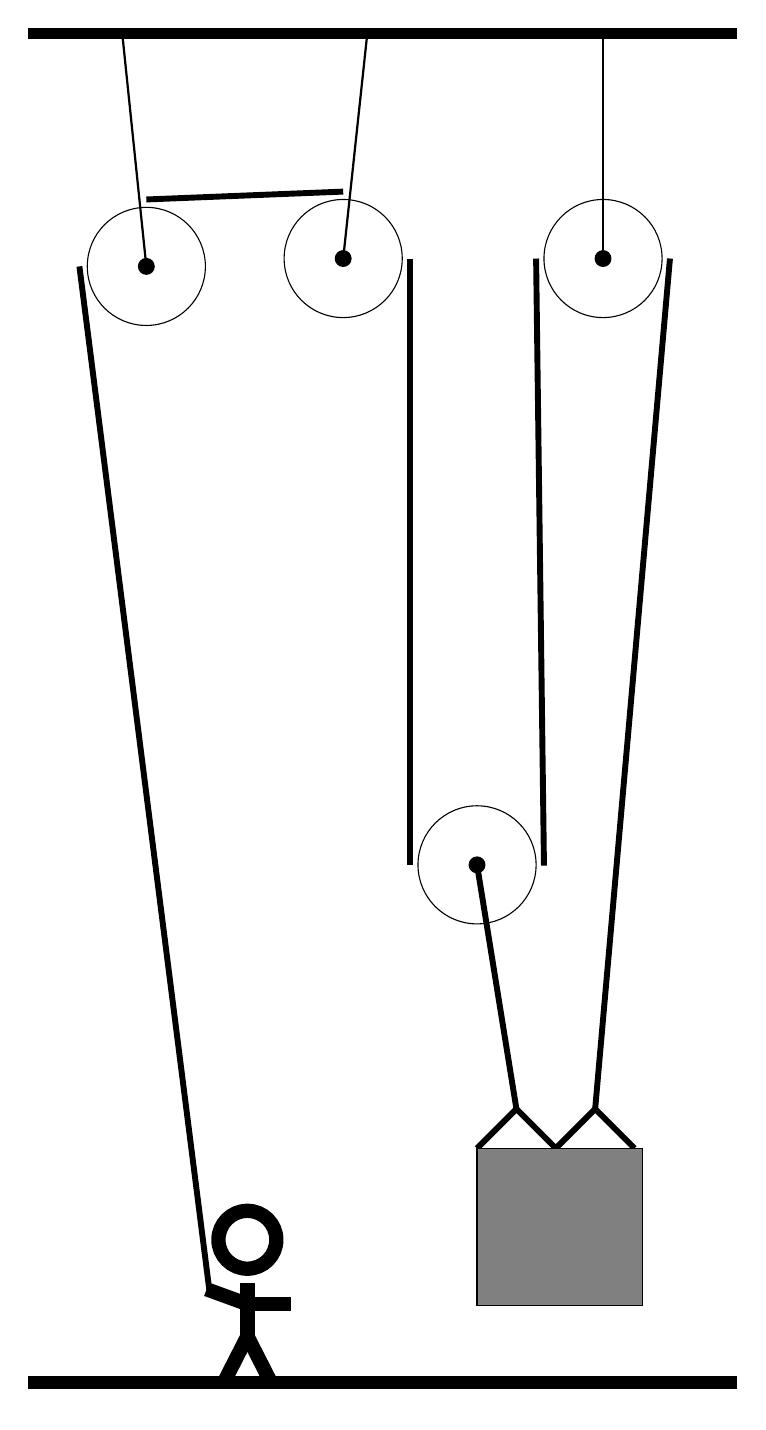
\begin{tikzpicture}
		%%%%% START %%%%%
		\draw[fill=black] (-3, 14) rectangle (6, 14.125);
		
		\draw (1, 11.2) circle (0.75);
		\draw[fill=black] (1, 11.2) circle (0.1);
		\draw[thick] (1, 11.2) -- (1.3, 14);
		
		\draw (4.3, 11.2) circle (0.75);
		\draw[fill=black] (4.3, 11.2) circle (0.1);
		\draw[thick] (4.3, 11.2) -- (4.3, 14);
		
		\draw (2.7, 3.5) circle (0.75);
		\draw[fill=black] (2.7, 3.5) circle (0.1);
		
		\draw[line width=0.75mm]  (2.7, -0.1) -- (3.2, 0.4) -- (3.7, -0.1) -- (4.2, 0.4) -- (4.7, -0.1);
		\draw[fill=black!50] (2.7, -0.1) rectangle (4.8, -2.1);
		
		\draw (-1.5, 11.1) circle (0.75);
		\draw[fill=black] (-1.5, 11.1) circle (0.1);
		\draw[thick] (-1.5, 11.1) -- (-1.8, 14);
		
		\draw[line width=0.75mm](-0.7, -1.9) --  (-2.35, 11.1);
		\centerarc[line width=0.75mm](-1.5, 11.1)(90:180:0.85);
		\draw[line width=0.75mm](-1.5, 11.95) -- (1, 12.05);
		\centerarc[line width=0.75mm](1, 11.2)(0:90:0.85);
		\draw[line width=0.75mm](1.85, 11.2) -- (1.85, 3.5);
		\centerarc[line width=0.75mm](2.7, 3.5)(180:370:0.85);
		\draw[line width=0.75mm] (3.55, 3.49) -- (3.45, 11.2);
		\centerarc[line width=0.75mm](4.3, 11.2)(0:180:0.85);
		\draw[line width=0.75mm](4.2, 0.4) -- (5.15, 11.2);
		\draw[line width=0.75mm] (3.2, 0.4) -- (2.7, 3.5);
		
		\node at (-0.2, -2) {\Strichmaxerl[10][-20][0]};
		
		\draw[fill=black] (-3, -3) rectangle (6, -3.15);
		%%%%% END %%%%%
	\end{tikzpicture}
\end{document}